\scanpage{32}\mspage{31}

If $A\in F\setminus G$, $A\cap B$ is a union of strata of $F$. \deleted{\unsure{Remains}} remains \unsure{to|:} see that a stratum \inserted{\unsure{$G$|$\in$|e}} of $F$ is a union of strata of $F'$. Let $A$ be this stratum of $F$. \deleted{\unsure{We|the|the}}
\[
 \deleted{A=\bigcup_{\substack{B\in F\\B\leq F}}B^\circ}
\]
If $A\notin G'$, \unsure{thus|then} $A\in F\setminus G'\subset F'$, and we win. If $A\in G$, then (since $G'\preceq G$) $A$ is a union of strata of $G'$, which are strata of $F'$, and we win again.

% slanted
\margin{Utterly false}
\uline{Corollary} The preceding \deleted{refinement}\inserted{subdivision} $F'$ of $F$ is characterized by \inserted{each} of the following \unsure{pr.|pro.} equivalent properties~:

\deleted{a) For every subdivision $F''$ of $F$ which induces $G'$ on $G$, we have $F''\preceq F'$ -- i.e. $F'$ is \deleted{\uline{maximal}}\inserted{a greatest \unsure{element|element|element}}, for $\preceq^{*}$, \unsure{in|for} the set of subdivisions of $F$ which induce $G'$ on $G$.}
% slanted
\margin{$*$ or for $\ll$, this amounts to the same among subdivisions of the same $F$}
% slanted; live state preferred, whole-note cancellation explicitly retained as an alternative.
\margin{\unsure{\figure{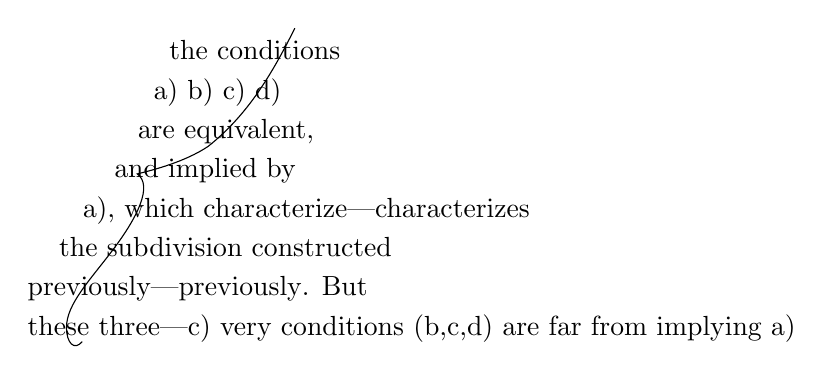
\begin{tikzpicture}[x=1mm,y=1mm,
 every node/.style={anchor=base west,inner sep=0pt}]
 \node at (18,0) {the conditions};
 \node at (16,-5) {\deleted{\unsure{a)}} b) c) d)};
 \node at (14,-10) {are equivalent,};
 \node at (11,-15) {\unsure{and} \uline{implied} by};
 \node at (7,-20) {a), which \unsure{characterize|characterizes}};
 \node at (4,-25) {the subdivision constructed};
 \node at (0,-30) {\unsure{previously|previously}. But};
 \node at (0,-35) {\unsure{these three|c) very} \unsure{conditions} (b,c,d) \unsure{are} \unsure{far} from implying a)};
 \draw (34,4)
  .. controls (31,-2) and (28,-7) .. (23,-11)
  .. controls (20,-13) and (16,-14) .. (14,-14.5)
  .. controls (16,-16) and (14,-20) .. (11,-24)
  .. controls (8,-28) and (5,-31) .. (5,-34)
  .. controls (5,-36) and (6,-37) .. (7,-35.8);
\end{tikzpicture}}|\deleted{the conditions \deleted{\unsure{a)}} b) c) d) are equivalent, \unsure{and} \uline{implied} by a), which \unsure{characterize|characterizes} the subdivision constructed \unsure{previously|previously}. But \unsure{these three|c) very} \unsure{conditions} (b,c,d) \unsure{are} \unsure{far} from implying a)}}}

% Small additional a)-like label above the end of application, attachment uncertain.
b) The canonical map \inserted{\unsure{a)}} associated with $F'\preceq F$
\[
 \varphi:F'\longrightarrow F
\]
induces a bijection
\[
 F'\setminus G'\xrightarrow{\sim}F\setminus G.
\]
\margin{\figure{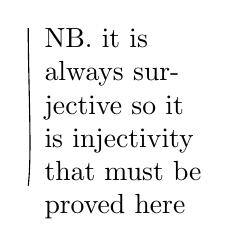
\begin{tikzpicture}[x=1mm,y=1mm]
 \draw (0,0) .. controls (0,-7) and (0.5,-16) .. (0,-20);
 \node[anchor=north west,inner sep=0pt,align=left,text width=20mm] at (2,0) {NB. it is always surjective so it is \uline{injectivity} that must be proved here};
\end{tikzpicture}}}

c) \deleted{The open strata of $F'$ which \unsure{are} not} \inserted{$\forall A\in F\setminus G$, $A^\circ$ is an open \unsure{stratum|stratum|stratum}} of $F'$.

d) $F'\supset F\setminus G$, i.e. $\forall A\in F\setminus G$, we have $A\in F'$.

\uline{Proof} We are going to prove for example
\[
 \text{d)}\Longrightarrow\text{b)}\Longrightarrow\text{c)}\Longrightarrow\text{a)}\Longrightarrow\text{d)}
\]
\deleted{\uline{\unsure{Proof}}} $\text{d)}\Rightarrow\text{b)}$ If $(F\setminus G)\subset F'$, then $\varphi\mid F\setminus G$ is the \deleted{\unsure{identity}}\inserted{canonical $F\setminus G\hookrightarrow F$} inclusion \deleted{(trivial)}, \deleted{therefore} therefore it remains to prove
\[
 F\setminus G=F'\setminus G'.
\]
